\documentclass[preprint]{elsarticle}

\usepackage{lineno,hyperref}
\modulolinenumbers[5]

\journal{Astroparticle Physics}

\bibliographystyle{elsarticle-num}%`Elsevier LaTeX' style

\begin{document}

\begin{frontmatter}

\title{The effective nucleon axial mass approach and quasielastic neutrino event rates in NO$\nu$A and Super-Kamiokande}

%% Group authors with affiliations in footnotes:
\author[ITEP,JINR]{K.~Kuzmin}
\ead{kkuzmin@theor.jinr.ru}

\author[JINR]{V.~Naumov}
\ead{vnaumov@theor.jinr.ru}

\author[JINR]{O.~Petrova\corref{correspondingauthor}}
\cortext[correspondingauthor]{Corresponding author}
\ead{redponick@gmail.com}

\author[JINR]{I.~Shandrov}
\ead{ishandrov@yahoo.co.uk}

\address[ITEP]{Institute for Theoretical and Experimental Physics, Bolshaya Cheremushkinskaya 25, RU-117218 Moscow, Russia}
\address[JINR]{Joint Institute for Nuclear Research, Joliot-Curie 6, RU-141980 Dubna, Russia}

\begin{abstract}
For the accurate interpretation of neutrino experiment results, in particular, for the neutrino mixing parameter extraction, it is necessary to study theoretical uncertainty in predicted count rates in detectors.

Quasielastic neutrino-nucleus interaction makes the main contribution to the count rate of so-called muon-like and electron-like events identified as single-ring events fully contained in water-Cherenckov detectors like Super-Kamiokande. Also quasielastic scattering events can be identified separately in tracking detectors, e.g. NO$\nu$A.

An essential source of calculation uncertainty belongs to cross sections of neutrino interactions with nucleons and nuclei. There is currently no generally accepted single nuclear model, applicable in a wide energy range, from threshold to extremely high values. Also there is a problem with nucleon structure functions, especially, with so-called nucleon axial mass, an important phenomenological parameter characterizing the axial-vector and pseudoscalar form factors. The range of quasielastic axial mass values used in the current Monte Carlo neutrino generators for a number of experiments \textbf{(from 0.99 GeV in T2K to 1.2 GeV in Super-Kamiokande)} seems to be unreasonably wide and distorting the interpretation of the experimental results.

Phenomenological solution for both these problems is to apply the effective axial mass, which means the use of the relativistic Fermi gas model of the nucleus at the same time with the introduction of the axial form factor parameterization. From the statistical analysis of available accelerator data on quasielastic neutrino scattering we extract the shape of the parameterization and optimal values of the parameters, which can be recommended for use in the neutrino generators.

\textbf{Brief alternative version}

In this study, we estimate the error in the quasielastic event rate prediction in experiments with atmospheric and accelerator neutrinos caused by the uncertainty in the value of the nucleon axial mass. It follows from our analysis that the impact of the axial mass uncertainty is comparable in magnitude with the expected neutrino oscillation effect itself. We propose a simple phenomenological method which allows to describe experimental quasielastic neutrino interaction data consistently and decrease uncertainty in the extracted neutrino mixing parameters.
\end{abstract}

\begin{keyword}
neutrino oscillation\sep quasielastic cross section\sep nucleon axial mass\sep Super-Kamiokande
\end{keyword}

\end{frontmatter}

\linenumbers

\section{Introduction: The axial mass problem}

The axial-vector and pseudoscalar form-factors in the electroweak nucleon current are the subject of long-standing theoretical and experimental efforts. However, these values still remain rather poorly known. Within the framework of the conventional parametrizations, both form-factors are characterized by a single phenomenological parameter, nucleon axial mass $M_A$:
\begin{equation}
F_{P}(Q^{2})={}\frac{2M^{2}}{m_{\pi}^{2}+Q^{2}}F_{A}(Q^{2}),\\
F_{A}(Q^{2})={}g_{A}\left(1+\frac{Q^{2}}{M_{A}^{2}}\right)^{-2},
\end{equation}
here $g_{A}=-1.2695$ --- axial-vector coupling, $m_{\pi}$ --- charged pion mass, $M=\frac{M_{n}+M_{p}}{2}$ --- isoscalar nucleon mass, $Q^{2}=-q^{2}$, where $q^{2}$ --- squared 4-momentum transfer.

Global statistical analysis of all available and mutually consistent data on the total and differential cross sections for the $\nu_{\mu}$ and $\bar\nu_{\mu}$ quasielastic scattering (QES) on different nuclear targets allows us to extract the best-fit value of nucleon axial mass: $M_A=0.95\pm0.06$\,GeV~\cite{Kuzmin:2007kr}. In Fig.~\ref{TotalCS} we demonstrate several examples of this analysis. The problem is in huge disagreement between the obtained best-fit value and the value extracted in the K2K and (especially) MiniBooNE experiments. Figures~\ref{K2K} and \ref{MiniBooNE} represent the K2K and the MiniBooNE measurements: $M_A=1.20\pm0.12$\,GeV~\cite{Gran:2006jn} and $M_{A}=1.35\pm0.17$\,GeV~\cite{AguilarArevalo:2010zc}, respectively. Thus, there is no consensus about right value of nucleon axial mass.

{\bf Figures}
\begin{figure}[h!]
\begin{center}
  \resizebox{18pc}{!}{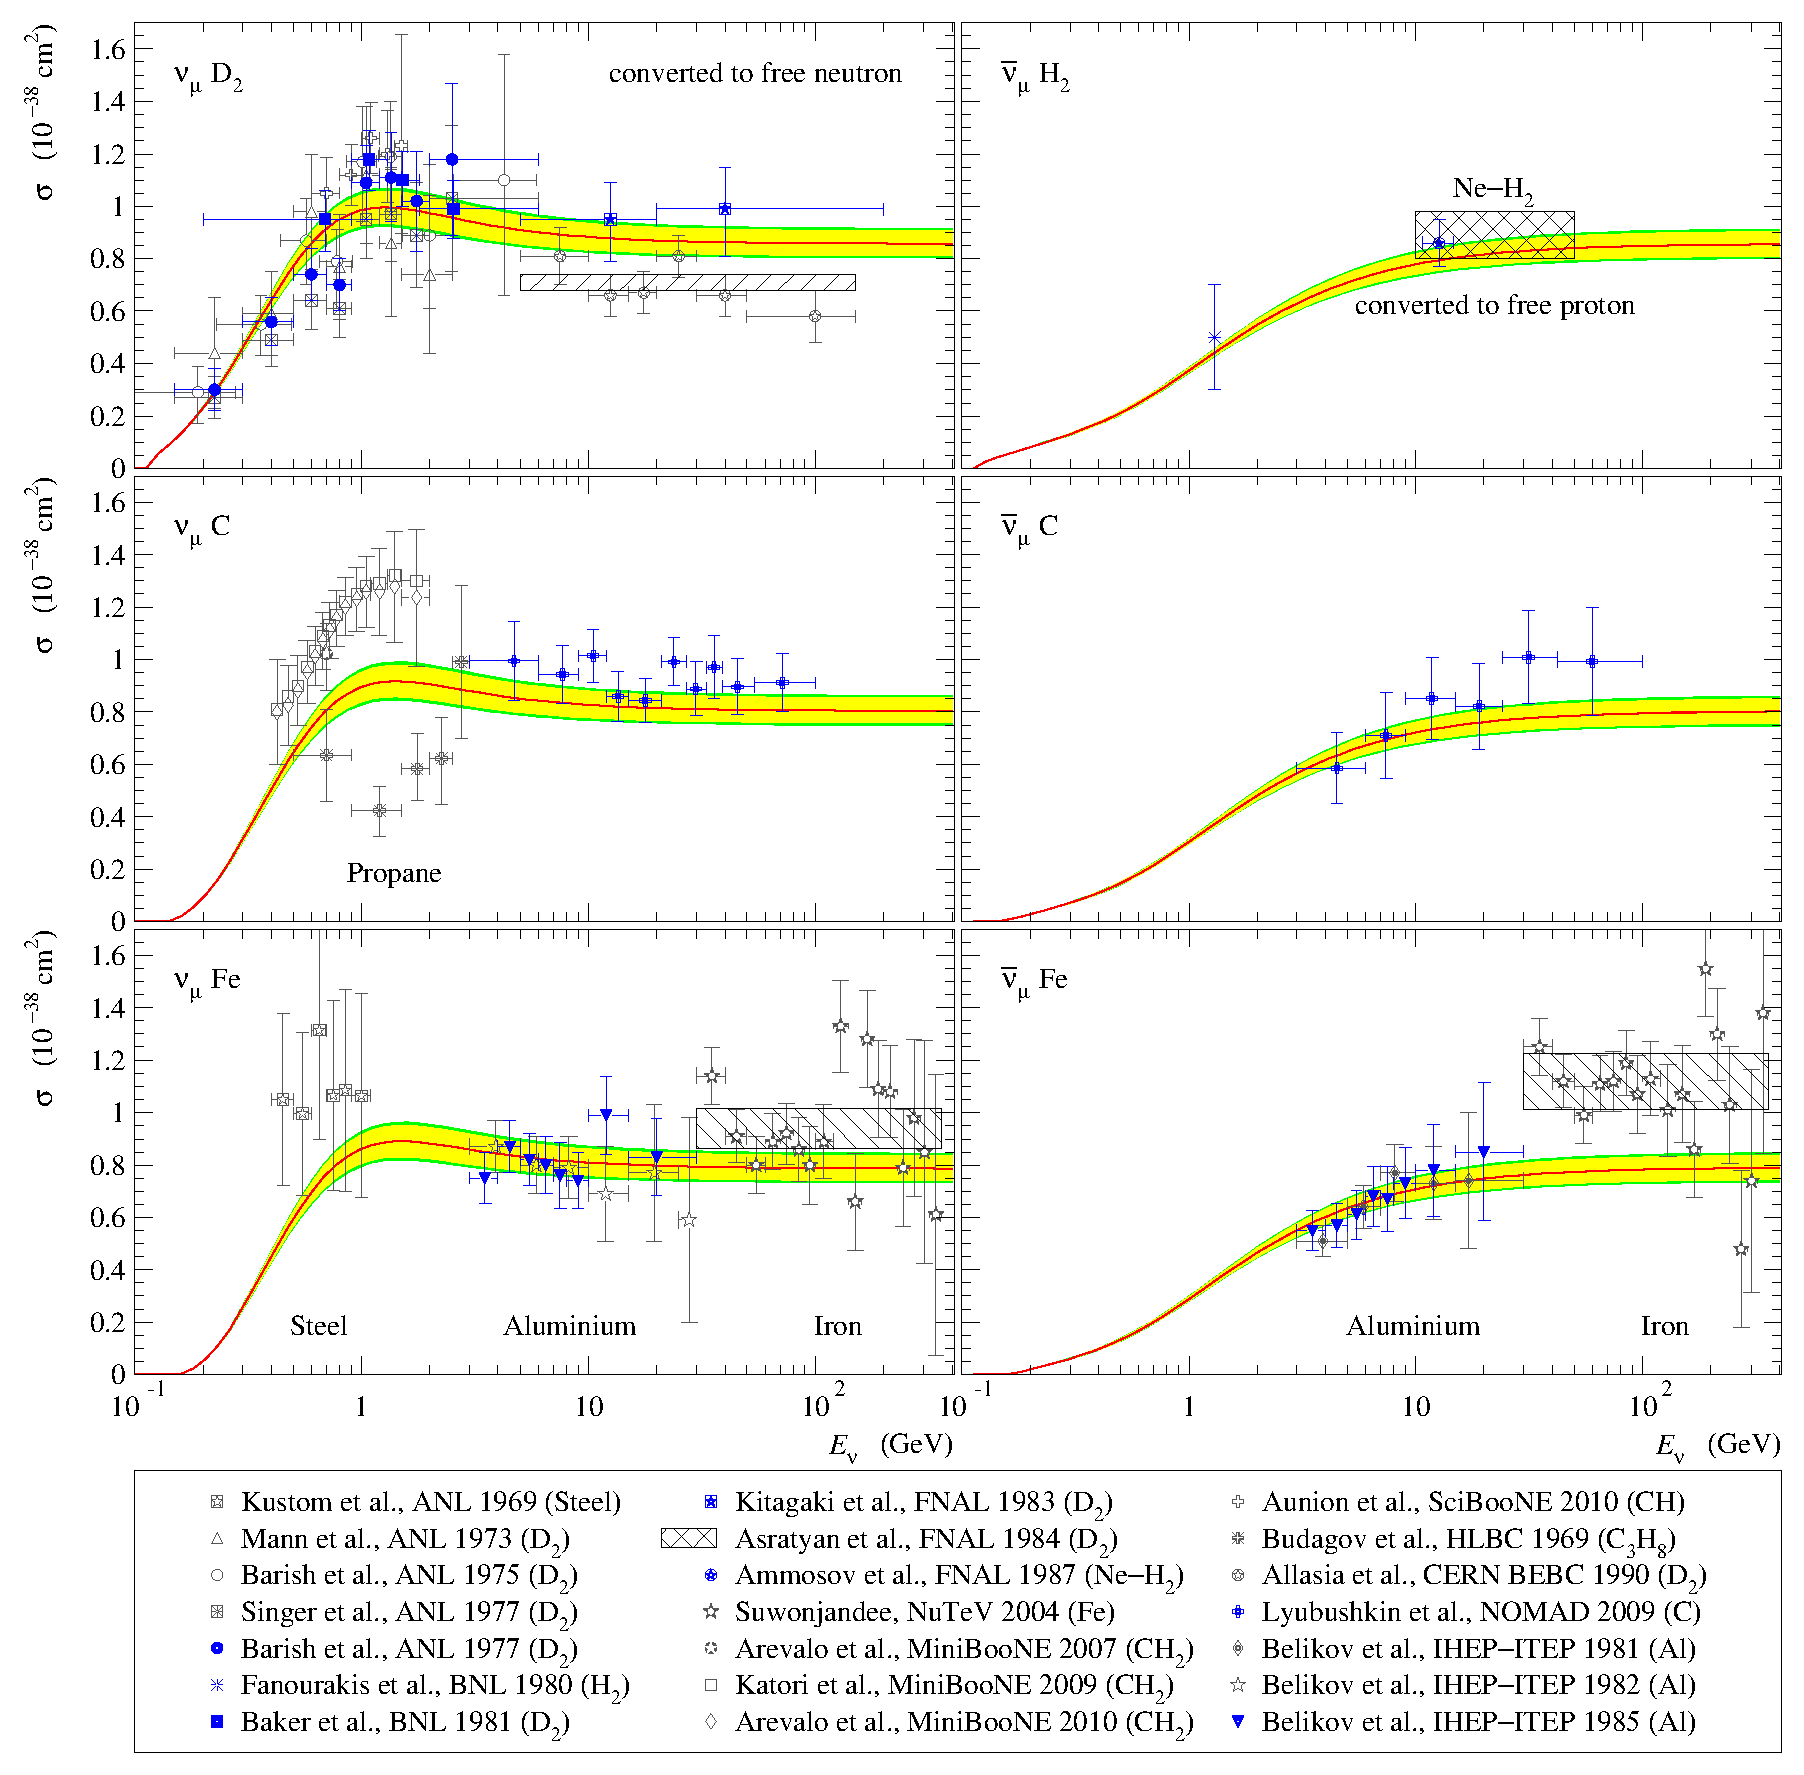
\includegraphics{./QES/sQESCC_101.3.00.301.00_2_BBBA25_NT_PART1.eps}}
  \resizebox{18pc}{!}{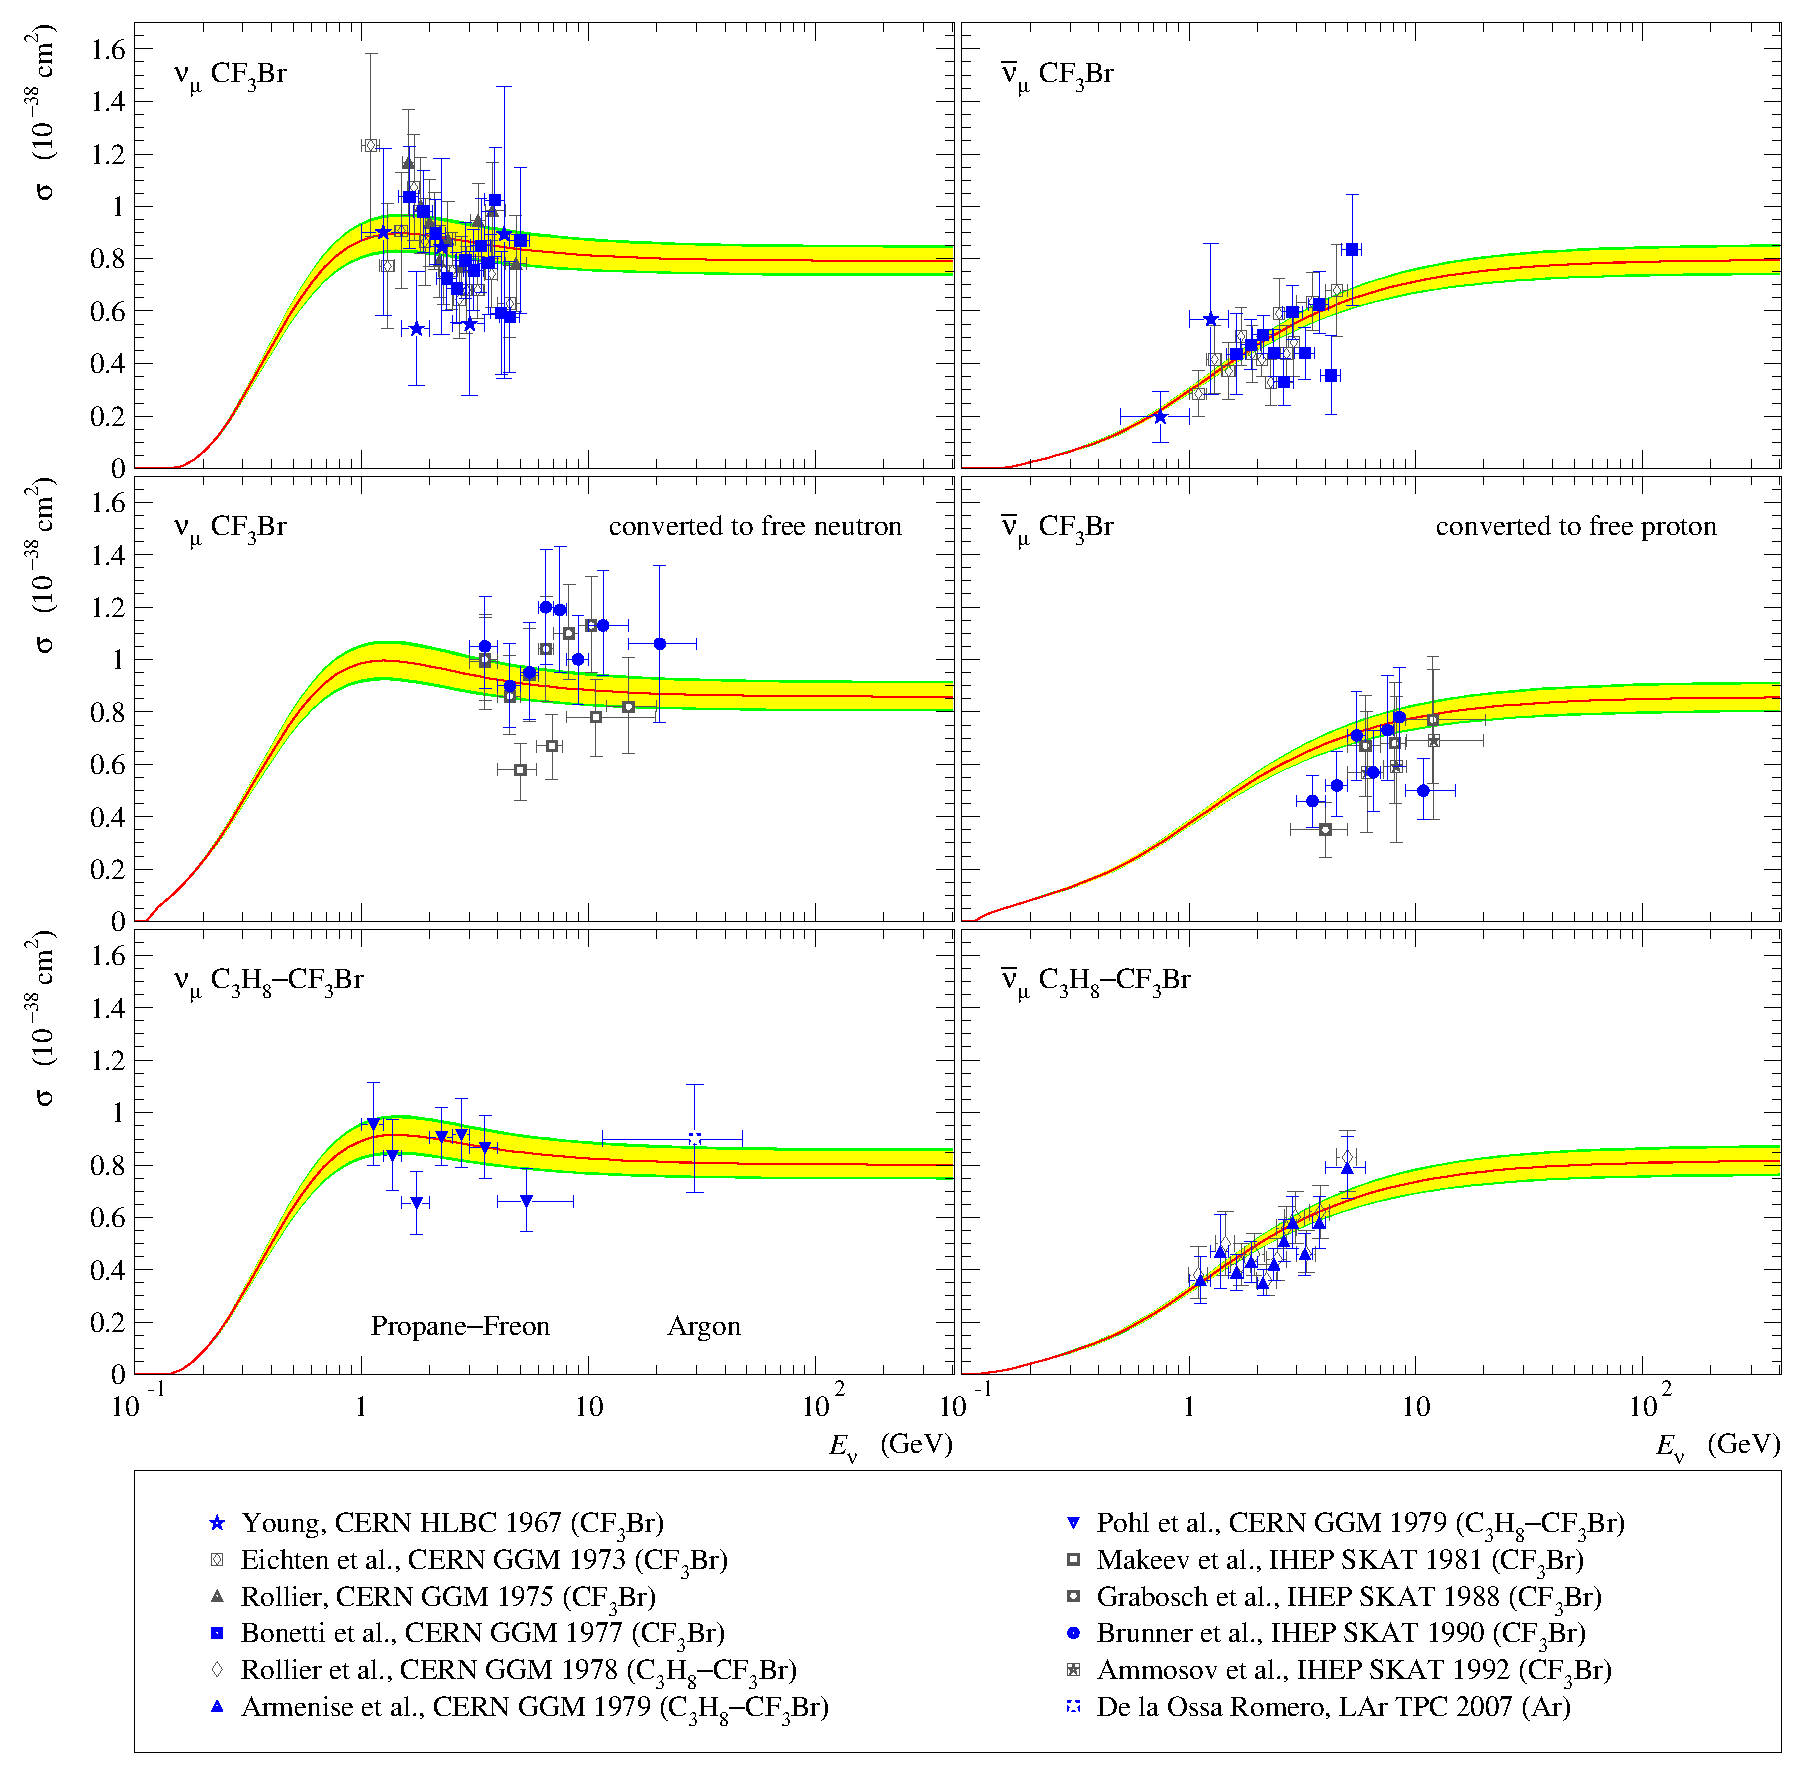
\includegraphics{./QES/sQESCC_101.3.00.301.00_2_BBBA25_NT_PART2.eps}}
\caption{\label{TotalCS}Total QES $\nu_{\mu}n$ \& $\bar\nu_{\mu}p$ cross sections measured in experiments with deuterium, hydrogen, carbon/propane, aluminium \& iron/steel targets (six left panels), and with freon \& propane-freon targets (six right panels). The curves show our current best-fit value. The widths of the inner (outer) bands correspond to the $1\sigma$ ($2\sigma$) standard deviations from the fit caused by the uncertainties in determination of $M_A$ including the spectrum normalizations. The light points are excluded from the global fit being either superseded by newer experiments, or not satisfying our selection criteria (see Ref.\cite{Kuzmin:2007kr} for more details and for the full set of the experimental data)}
\end{center}
\end{figure}

\begin{figure}[h!]
\begin{center}
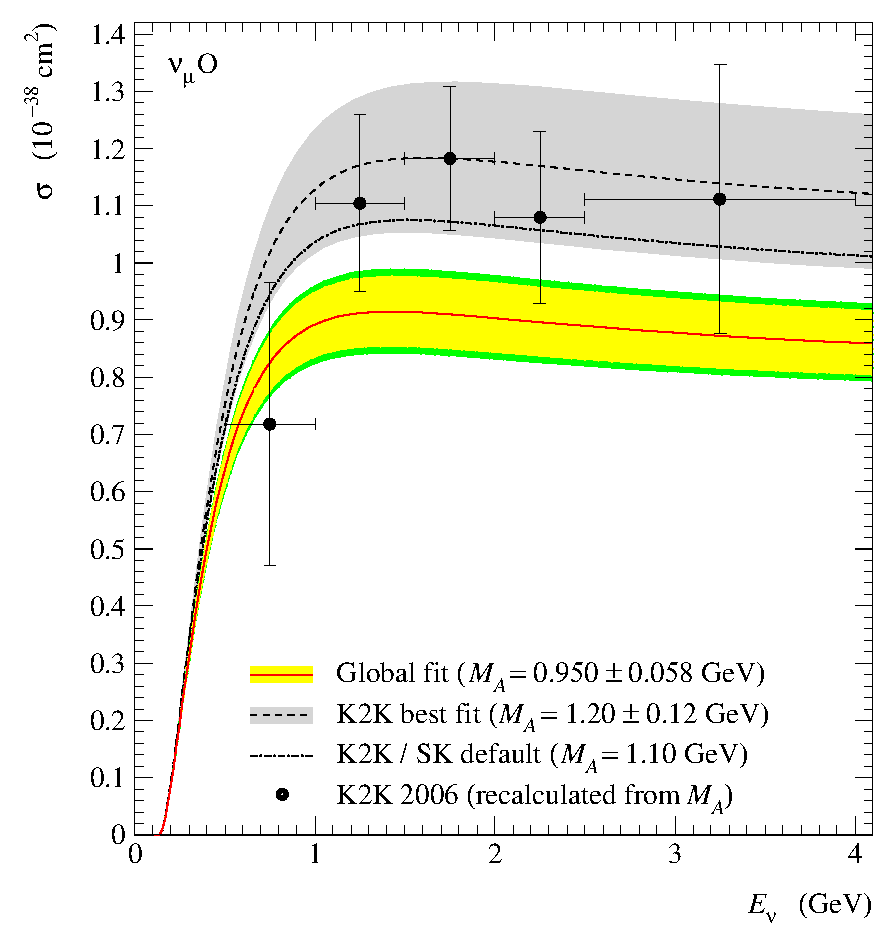
\includegraphics[width=0.45\textwidth]{./QES/sQESCC_K2K06_101.3.00.301.00_2_BBBA25_SM.eps}
\caption{\label{K2K}A comparison of the QES $\nu_{\mu}$ cross sections per neutron bound in oxygen evaluated with different values of $M_A$. The dashed curve with accompanying band corresponds to the K2K extraction of $M_A$~\cite{Gran:2006jn}. The dash-dotted curve is the cross section calculated with $M_A=1.1$\,GeV, the value which was the K2K and SK\,I default before 2006~\cite{Gran:2006jn,Ashie:2005ik}. The points in Fig.~\ref{K2K} represent the total QES cross section reconstructed from the ``raw'' K2K data}
\end{center}
\end{figure}

\begin{figure}[h!]
\begin{center}
  \resizebox{18pc}{!}{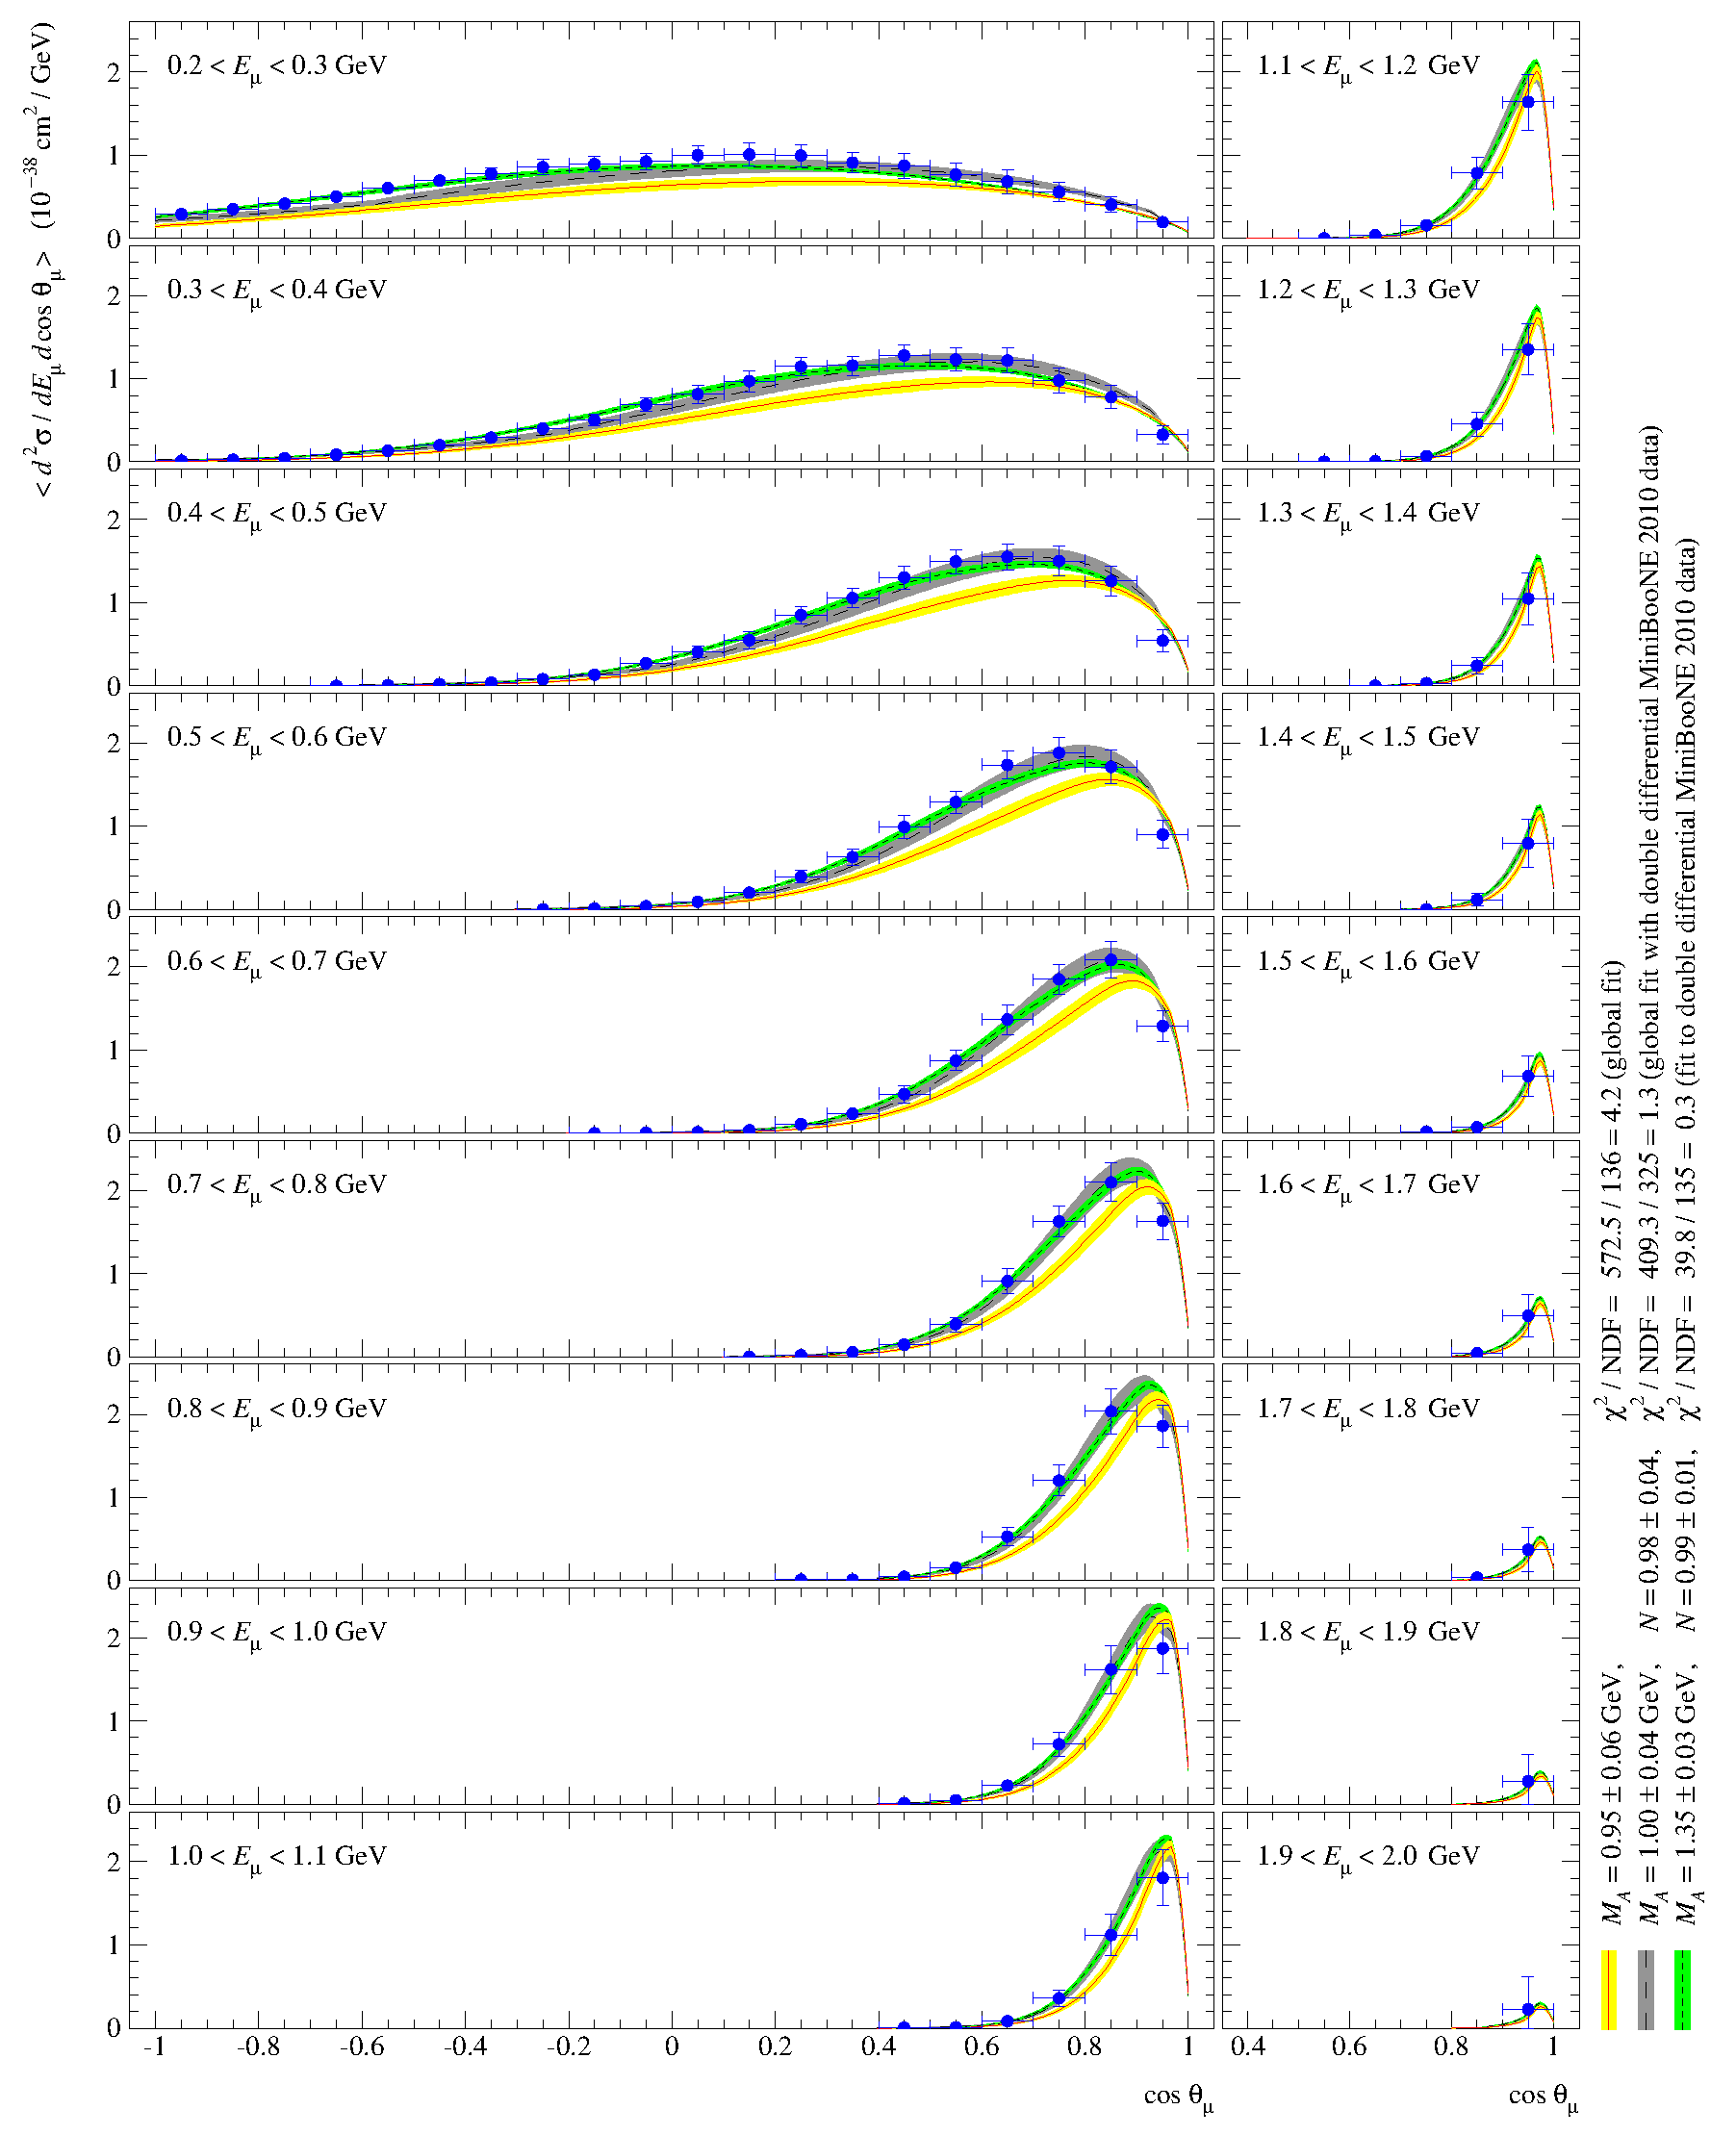
\includegraphics{./QES/d2sQESCC_dEkdcosT_Arevalo_MiniBooNE10_Ek_2_BBBA25.eps}}
  \resizebox{18pc}{!}{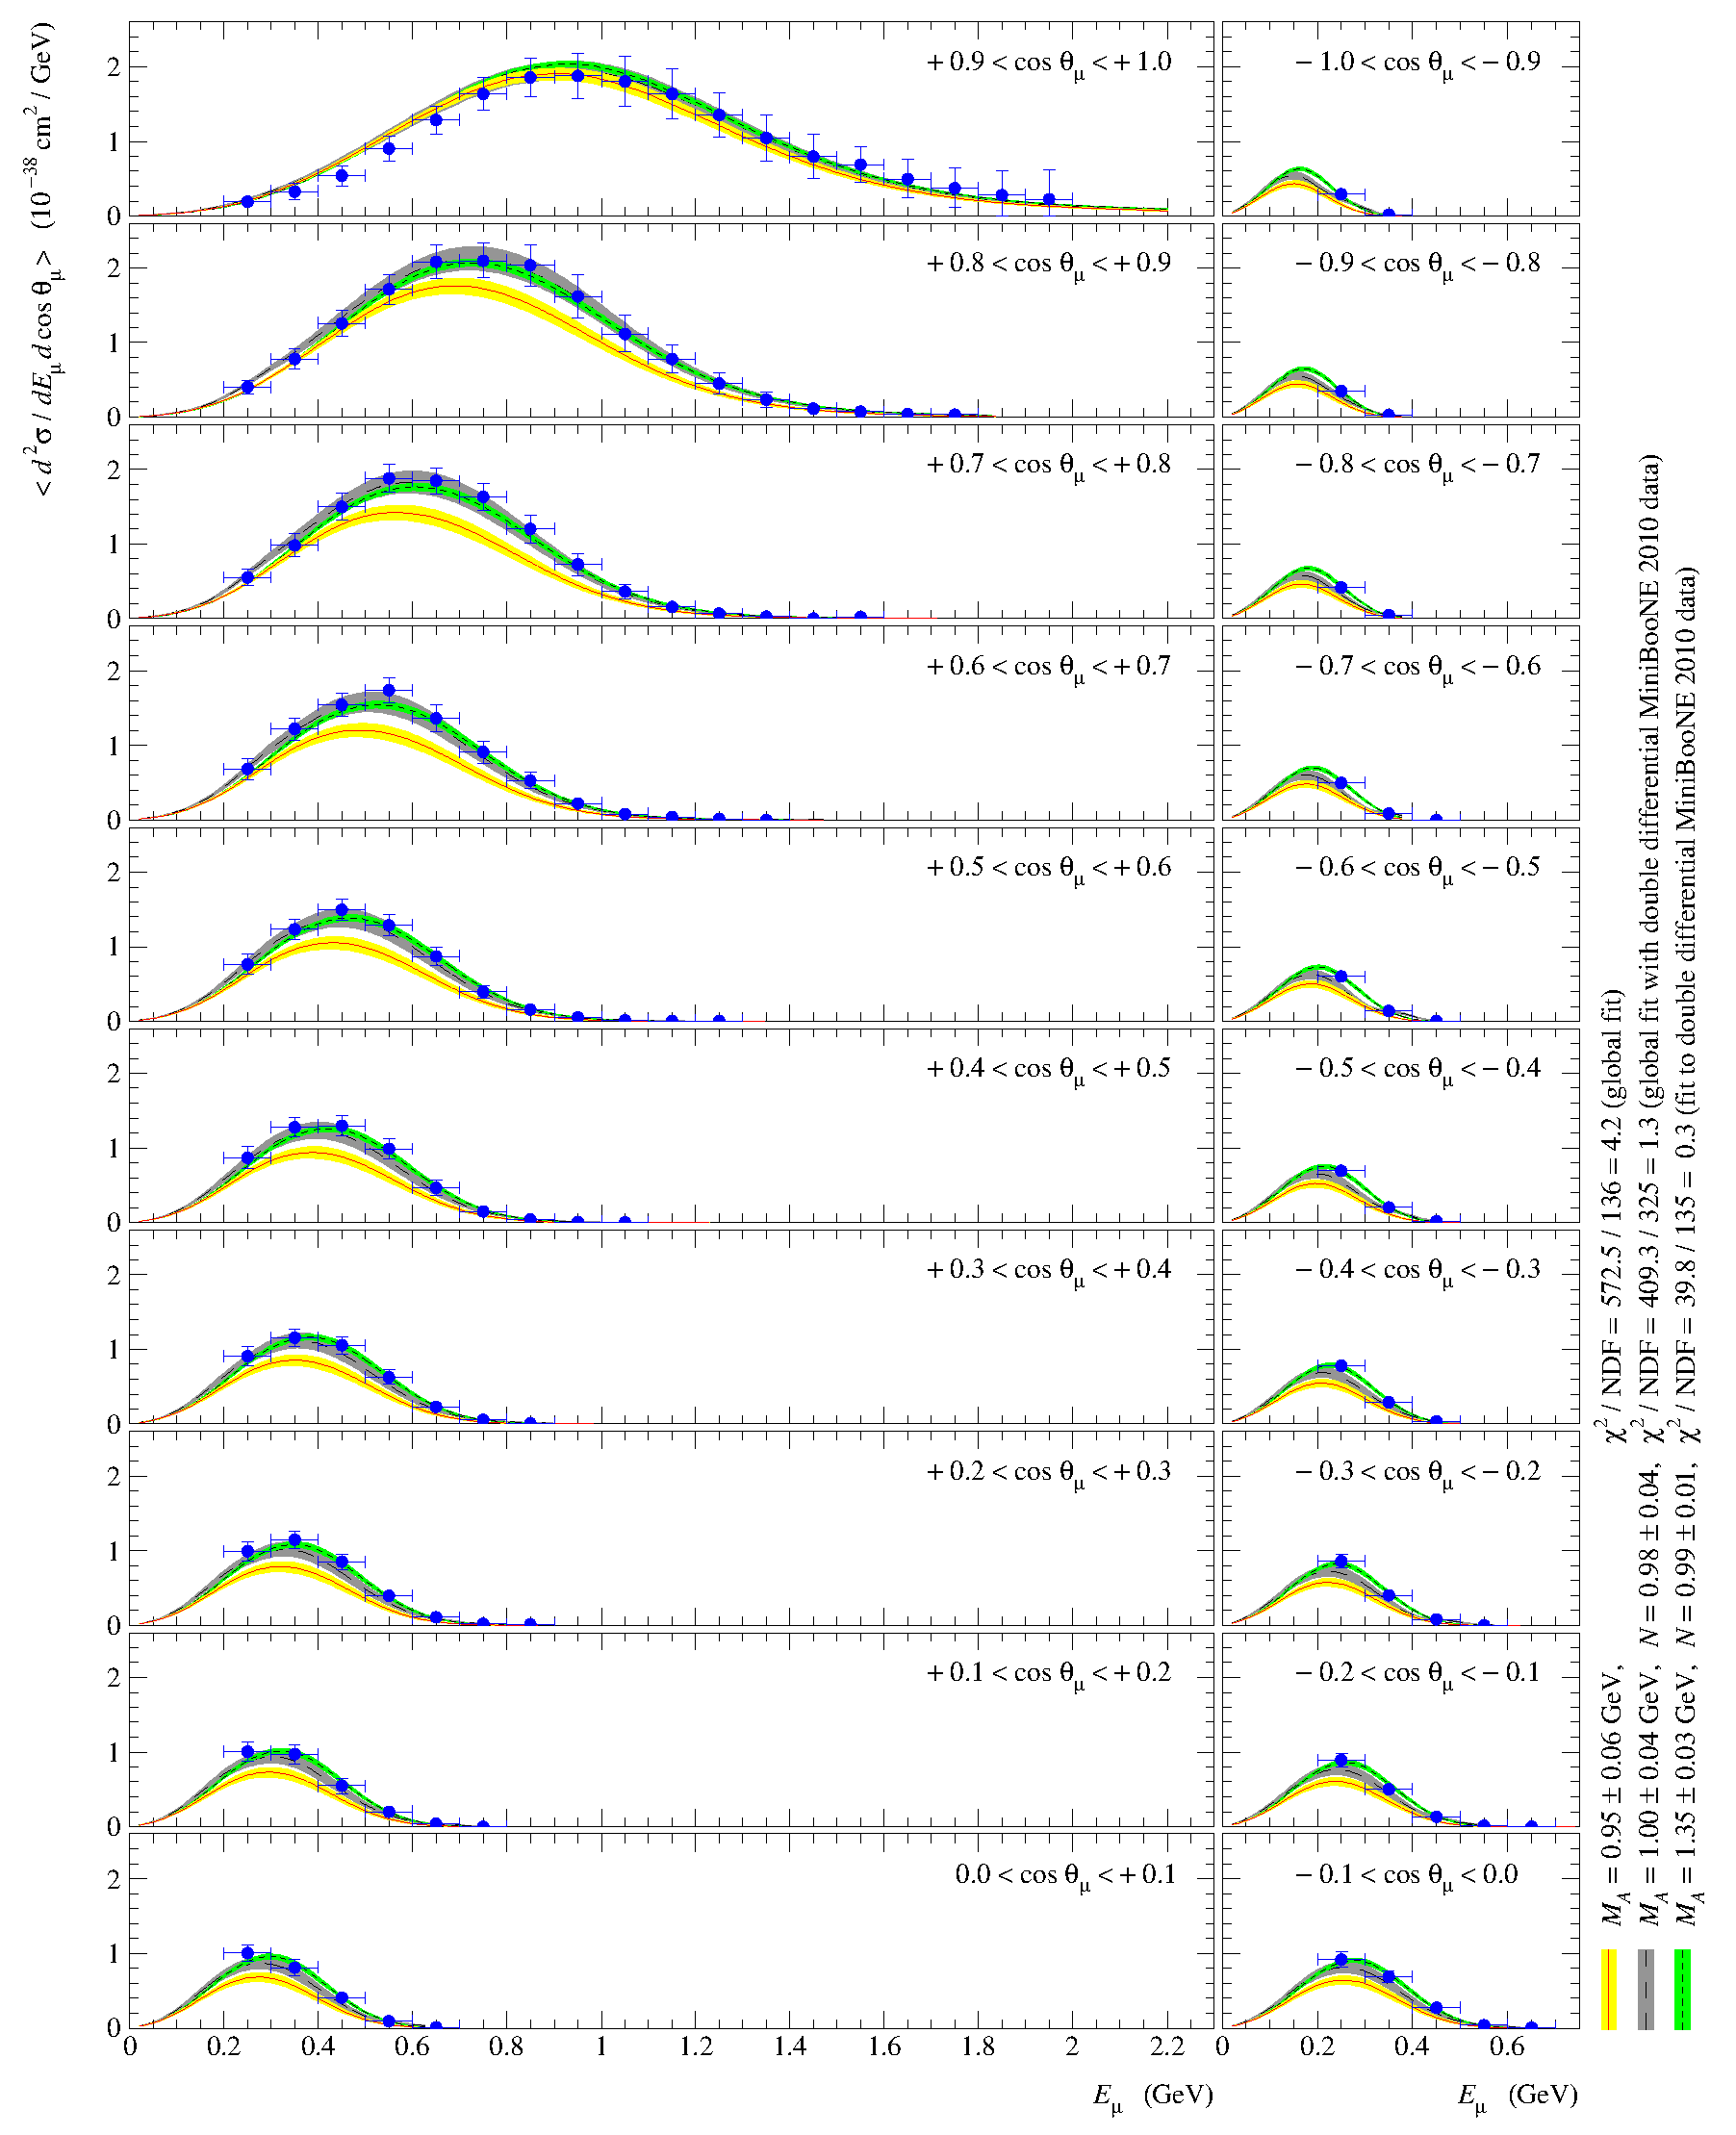
\includegraphics{./QES/d2sQESCC_dEkdcosT_Arevalo_MiniBooNE10_cosT_2_BBBA25.eps}}
\caption{\label{MiniBooNE}The flux-weighted double differential cross sections for the $\nu_{\mu}n\to\mu^-p$ reaction measured in the high-statistics experiment MiniBooNE filled with undoped mineral oil (CH$_2$) and exposed to FNAL Booster Neutrino Beam at Fermilab~\cite{AguilarArevalo:2010zc}. The meaning of the bands and corresponding curves is clear from the legends on the right. The dark bands are calculated by using the nuclear model of Martini \textit{et al.}~\cite{Martini:2011wp}, which yields $M_A$ compatible with our best-fit value obtained without the MiniBooNE dataset}
\label{MiniBooNE}
\end{center}
\end{figure}

Let us stress that the exact knowledge of axial mass is needed for many applications in neutrino physics and astrophysics. In particular, it is important for the data processing of the neutrino oscillation experiments with (anti)neutrinos from accelerators and cosmic rays. The aim of this paper is to investigate the impact of the uncertainty in $M_A$ on the predicted event rates in the underground neutrino detectors. As a major example we consider the World's largest detector Super-Kamiokande.

\section{Methodology}
\subsection{Atmospheric neutrinos}
Atmosperic neutrinos are produced by the interaction of cosmic rays with the upper atmosphere. In the subsequent calculations we used the most recent 3D Monte Carlo calculations by Honda \textit{et al.}~\cite{Honda:2011nf}. This model is based on the nuclear interaction model JAM used in Particle and Heavy-Ion Transport code System and modified DPMJET-III package.
%Geomagnetic cutoff at Kamioka site is considered.
\subsection{Neutrino oscillations}
Atmosperic neutrino fluxes are modified by neutrino oscillation phenomenon. For computing the flavor transition and survival probabilities we applied the result of the global neutrino oscillation data analysis~\cite{Tortola:2012te} (the relevant values of the neutrino mixing angles, CP violating phase and squared mass splittings are listed in Table~\ref{tab:NOP}).
\begin{table}[!ht]
\begin{center}
\caption{\label{tab:NOP}\small Neutrino mixing parameters for normal (upper rows) and inverse (lower rows) neutrino mass hierarchy.}
\vspace{2mm}
{\small
\begin{tabular}{|c|c|c|c|c|}
\hline
parameter	&best fit	&$1\sigma$	&$2\sigma$	&$3\sigma$\\
\hline
\begin{tabular}{c}
$\Delta{m}^{2}_{21}$\\
$[10^{-5}\mathrm{eV}^{2}]$
\end{tabular}	&$7.62$	&$7.43-7.81$	&$7.27-8.01$	&$7.12-8.20$\\[3mm]
\begin{tabular}{c}
$|\Delta{m}^{2}_{31}|$\\
$[10^{-3}\mathrm{eV}^{2}]$
\end{tabular}
	&\begin{tabular}{c}
		$2.55$\\
		$2.43$
	\end{tabular}	
	&\begin{tabular}{c}
		$2.46-2.61$\\
		$2.37-2.50$
	\end{tabular}
	&\begin{tabular}{c}
		$2.38-2.68$\\
		$2.29-2.58$
	\end{tabular}	
	&\begin{tabular}{c}
		$2.31-2.74$\\
		$2.21-2.64$
	\end{tabular}\\[3mm]
$\sin^{2}\theta_{12}$	&$0.320$	&$0.303-0.336$	&$0.29-0.35$	&$0.27-0.37$\\[3mm]
$\sin^{2}\theta_{23}$	
	&\begin{tabular}{c}
		$0.613$\\
		$0.600$
	\end{tabular}
	&\begin{tabular}{c}
		$0.400-0.461\cup0.573-0.635$\\
		$0.569-0.626$
	\end{tabular}
	&\begin{tabular}{c}
		$0.38-0.66$\\
		$0.39-0.65$
	\end{tabular}
	&\begin{tabular}{c}
		$0.36-0.68$\\
		$0.37-0.67$
	\end{tabular}\\[5mm]
$\sin^{2}\theta_{13}$	
	&\begin{tabular}{c}
		$0.0246$\\
		$0.0250$
	\end{tabular}
	&\begin{tabular}{c}
		$0.0218-0.0275$\\
		$0.0223-0.0276$
	\end{tabular}
	&\begin{tabular}{c}
		$0.019-0.030$\\
		$0.020-0.030$
	\end{tabular}	&$0.017-0.033$\\[3mm]
$\delta$	
	&\begin{tabular}{c}
		$0.80\pi$\\
		$-0.03\pi$
	\end{tabular}
	&$0-2\pi$	&$0-2\pi$	&$0-2\pi$\\[3mm]
\hline
\end{tabular}}
\end{center}
\vspace{-0.5cm}
\end{table}

\subsection{Earth's profile}
Before getting the detector, neutrinos pass through the body of the Earth. Therefore, we had to take into account the neutrino-matter coherent scattering (MSW effect). To solve the Wolfenstein equations we used the method of Ref.~\cite{Naumov:1991ju,Naumov:1991rh}. The density profile in the Earth in the presented calculations is described according to the Two-Layer Earth Model (2LEM)~\cite{Agarwalla:2012uj}.

\section{Results and discussion: The axial mass effect}
Figure~\ref{CountRate} demonstrates the result of our calculation: the relative contributions to the electron-like and muon-like event rates caused by the QES interactions with hydrogen and oxygen nuclei in the Super-Kamiokande detector. Evaluations were done with several values of nucleon axial mass and normalized to one of them. As you can see, the adequate choice of the axial mass value is very important to the neutrino event rate calculations.

\begin{figure}[h!]
\begin{center}
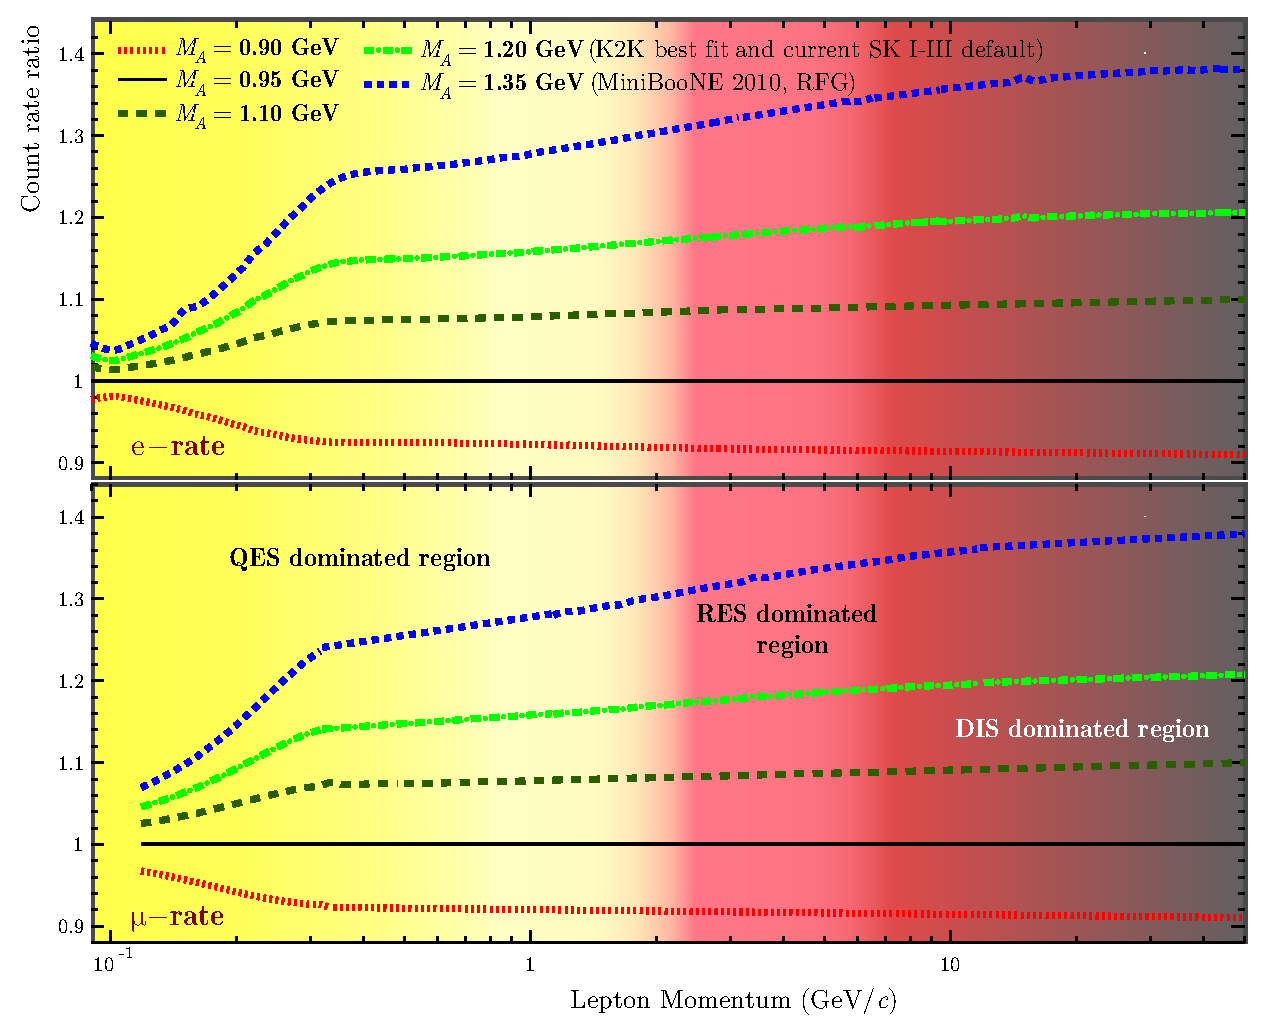
\includegraphics[width=0.45\textwidth]{./SK/Count_rate_ratio.eps}
\caption{\label{CountRate}Electron and muon count rates in the Super-Kamiokande detector due to QES interactions evaluated with different values of $M_A$ and normalized to one of them. The calculations are done for the normal neutrino mass hierarchy. Energy regions, where quasielastic, resonant or deep inelastic scattering are dominant, are shown approximate}
\end{center}
\end{figure}

A nuclear model commonly used in experiments for data processing is the Relativistic Fermi Gas model. All of experimantal data mentioned in Introduction were obtained by using this model. Applying another model could essentially modify extracted values. Figure~\ref{MiniBooNE} shows calculation exploiting the nuclear model of Martini \textit{et al.}~\cite{Martini:2011wp}, which yields $M_A$ compatible with our best-fit value. The natural conclusion is that the Relativistic Fermi Gas model does not work in the low-energy region. The problem is that we don't have nuclear model, which works properly for all energies. Therefore, even in case we knew the correct value of the axial mass, we could not use it.

But finally, we have an idea of how to avoid this difficulty. As we know, using the RFG model with different values of $M_A$ can give a good description of experimental data obtained in different energy ranges. Thus, we propose to continue using the Relativistic Fermi Gas model but modify the axial form factor to compensate nuclear effects in the low-energy region. For this parametrization we need to introduce variable effective axial mass:
\begin{equation}
F_{A}^{\mathrm{eff}}(Q^{2},E_{\nu})=g_{A}\left(1+\frac{Q^{2}}{(M_{A}^{\mathrm{eff}}(E_{\nu}))^{2}}\right)^{-2}.
\end{equation}
Figure~\ref{MA_QES_Effective} demonstrates very schematically how we can fit experimental data to get $M_{A}^{\mathrm{eff}}$. In the near future we plan to perform a global statistical analisys to adjust $M_{A}^{\mathrm{eff}}$.

\begin{figure}[h!]
\begin{center}
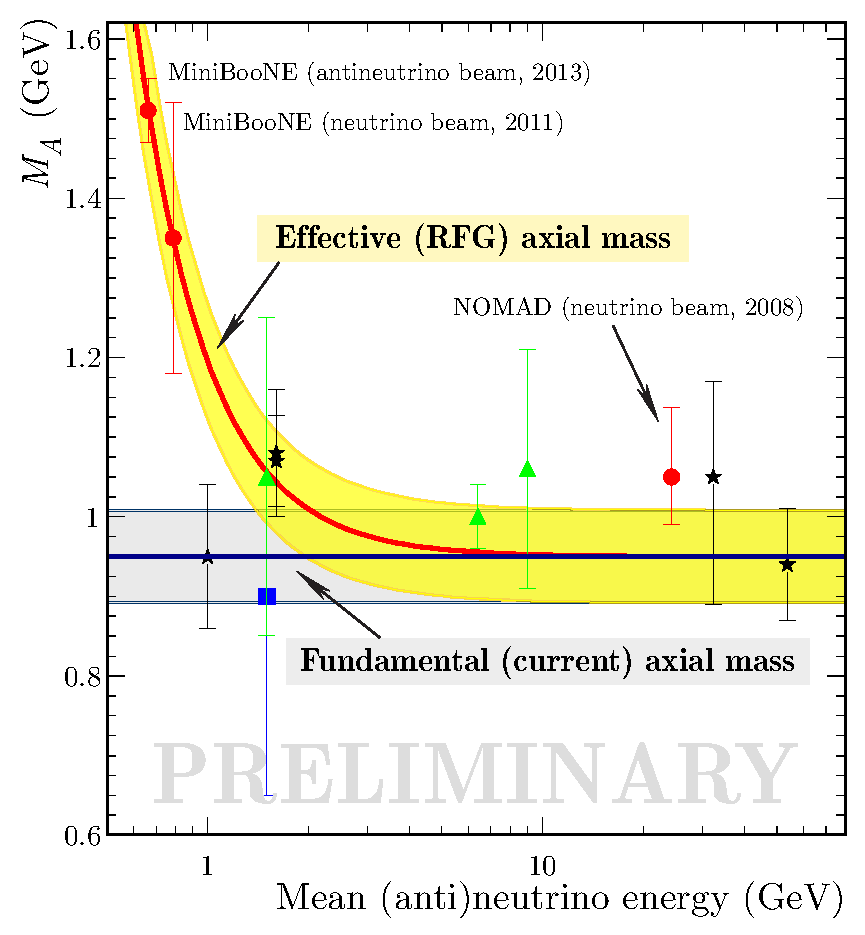
\includegraphics[width=0.45\textwidth]{./QES/MA_QES_Effective-2.eps}
\caption{\label{MA_QES_Effective}The concept of how we can fit experimental data to get $M_{A}^{\mathrm{eff}}$. Only selected experimental points are shown. Only MininBooNE data are used to fit the $M_{A}^{\mathrm{eff}}$ curve}
\end{center}
\end{figure}

In contrast, we propose to call constant $M_A$ used in real form-factor $F_A$ ``current''. Figure~\ref{EventRates} displays ratios of the neutrino event rates evaluated with several values of current $M_A$ to ones computed with preliminary offered $M_{A}^{\mathrm{eff}}$.

\begin{figure}[h!]
\begin{center}
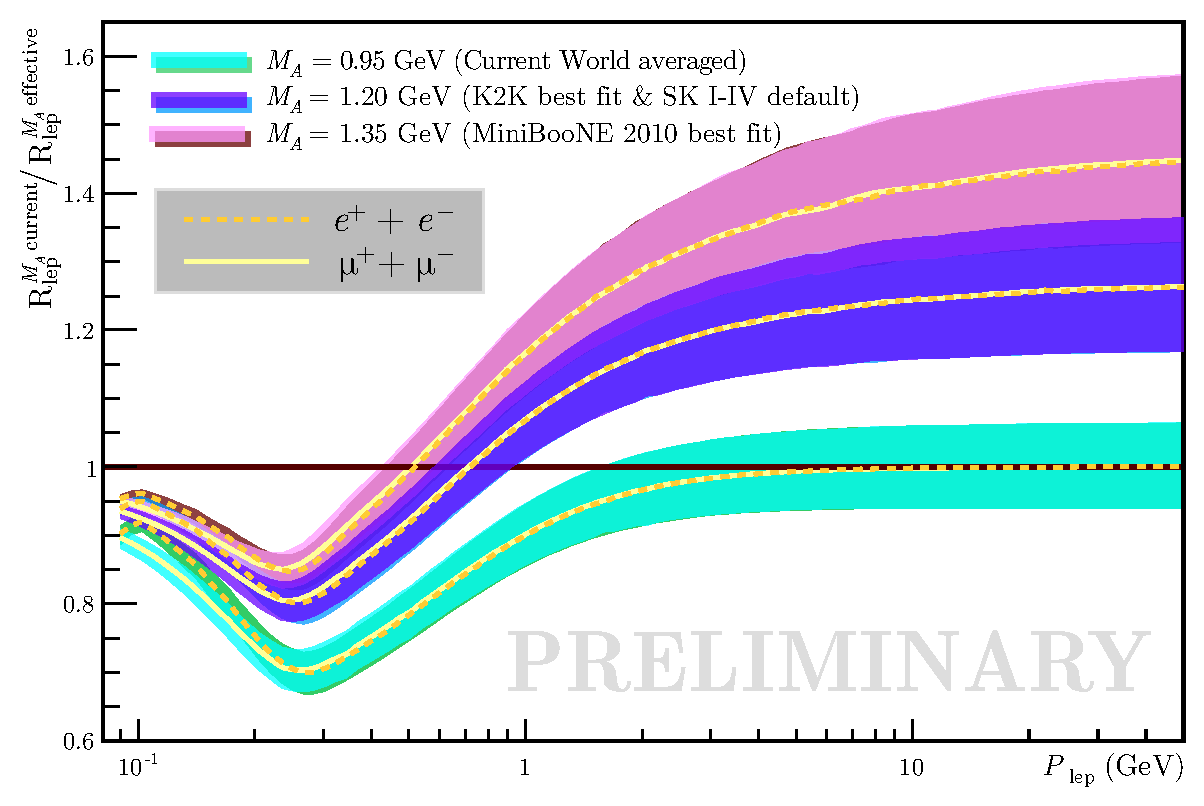
\includegraphics[width=0.45\textwidth]{./SK/cvsv2lmn_all2.eps}
\caption{\label{EventRates}Electron-like and muon-like event rates caused by the QES interactions in the SK detector. The rates are evaluated with several values of current $M_A$ and normalized to the rates calculated with the effective $M_A$. The calculations are done for the normal neutrino mass hierarchy}
\end{center}
\end{figure}

\section{Conclusions}
In this paper we demonstrated that the choice of the nucleon axial mass value essentially affects the predicted count rates in the Super-Kamiokande detector particularly within the region, which the QES interactions are dominant in. The related uncertainty is comparable with that in the predicted atmospheric neutrino fluxes, as well as with the scale of the oscillation effect itself. Hence, the effect should be taken into account for the correct determination of the neutrino mixing parameters. 

Let us emphasize the fact that the estimations presented herein are preliminary. However, we believe that using the effective axial mass instead of the value 1.2\,GeV currently used by the SK Collaboration~\cite{Wendell:2010md} or the value $0.99$\,GeV used by the T2K Collaboration~\cite{Abe:2011ks} should substantially improve the validity of the extracted neutrino mixing parameter values.

Future progress in the nuclear modelling and new experiments (e.g., MINER$\nu$A) will hopefully allow us to improve the accuracy of the current $M_A$ extraction and $M_{A}^{\mathrm{eff}}$ determination.

\section*{References}
\bibliography{bibfile}

\end{document}
